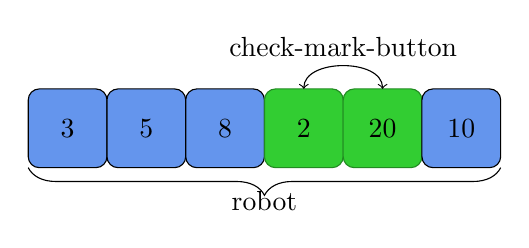
\begin{tikzpicture}
\node[draw=Black, fill=CornflowerBlue, rounded corners, minimum width=1cm, minimum height=1cm] at (0, 0) {3};
\node[draw=Black, fill=CornflowerBlue, rounded corners, minimum width=1cm, minimum height=1cm] at (1, 0) {5};
\node[draw=Black, fill=CornflowerBlue, rounded corners, minimum width=1cm, minimum height=1cm] at (2, 0) {8};
\node[draw=ForestGreen, fill=LimeGreen, rounded corners, minimum width=1cm, minimum height=1cm] at (3, 0) {2};
\node[draw=ForestGreen, fill=LimeGreen, rounded corners, minimum width=1cm, minimum height=1cm] at (4, 0) {20};
\node[draw=Black, fill=CornflowerBlue, rounded corners, minimum width=1cm, minimum height=1cm] at (5, 0) {10};
\path[<->] (3, .5) edge[bend left=90] node [above]{\emoji{check-mark-button}} (4, 0.5);
\draw[decorate,decoration={brace,mirror,amplitude=10pt}] (-0.5,-.5) -- (5.5,-.5) node[midway, below=5pt] {\emoji{robot}};
\end{tikzpicture}\caption{Schritt 5 (ausgetauscht!)}
